\documentclass[1p]{elsarticle_modified}
%\bibliographystyle{elsarticle-num}

%\usepackage[colorlinks]{hyperref}
%\usepackage{abbrmath_seonhwa} %\Abb, \Ascr, \Acal ,\Abf, \Afrak
\usepackage{amsfonts}
\usepackage{amssymb}
\usepackage{amsmath}
\usepackage{amsthm}
\usepackage{scalefnt}
\usepackage{amsbsy}
\usepackage{kotex}
\usepackage{caption}
\usepackage{subfig}
\usepackage{color}
\usepackage{graphicx}
\usepackage{xcolor} %% white, black, red, green, blue, cyan, magenta, yellow
\usepackage{float}
\usepackage{setspace}
\usepackage{hyperref}

\usepackage{tikz}
\usetikzlibrary{arrows}

\usepackage{multirow}
\usepackage{array} % fixed length table
\usepackage{hhline}

%%%%%%%%%%%%%%%%%%%%%
\makeatletter
\renewcommand*\env@matrix[1][\arraystretch]{%
	\edef\arraystretch{#1}%
	\hskip -\arraycolsep
	\let\@ifnextchar\new@ifnextchar
	\array{*\c@MaxMatrixCols c}}
\makeatother %https://tex.stackexchange.com/questions/14071/how-can-i-increase-the-line-spacing-in-a-matrix
%%%%%%%%%%%%%%%

\usepackage[normalem]{ulem}

\newcommand{\msout}[1]{\ifmmode\text{\sout{\ensuremath{#1}}}\else\sout{#1}\fi}
%SOURCE: \msout is \stkout macro in https://tex.stackexchange.com/questions/20609/strikeout-in-math-mode

\newcommand{\cancel}[1]{
	\ifmmode
	{\color{red}\msout{#1}}
	\else
	{\color{red}\sout{#1}}
	\fi
}

\newcommand{\add}[1]{
	{\color{blue}\uwave{#1}}
}

\newcommand{\replace}[2]{
	\ifmmode
	{\color{red}\msout{#1}}{\color{blue}\uwave{#2}}
	\else
	{\color{red}\sout{#1}}{\color{blue}\uwave{#2}}
	\fi
}

\newcommand{\Sol}{\mathcal{S}} %segment
\newcommand{\D}{D} %diagram
\newcommand{\A}{\mathcal{A}} %arc


%%%%%%%%%%%%%%%%%%%%%%%%%%%%%5 test

\def\sl{\operatorname{\textup{SL}}(2,\Cbb)}
\def\psl{\operatorname{\textup{PSL}}(2,\Cbb)}
\def\quan{\mkern 1mu \triangleright \mkern 1mu}

\theoremstyle{definition}
\newtheorem{thm}{Theorem}[section]
\newtheorem{prop}[thm]{Proposition}
\newtheorem{lem}[thm]{Lemma}
\newtheorem{ques}[thm]{Question}
\newtheorem{cor}[thm]{Corollary}
\newtheorem{defn}[thm]{Definition}
\newtheorem{exam}[thm]{Example}
\newtheorem{rmk}[thm]{Remark}
\newtheorem{alg}[thm]{Algorithm}

\newcommand{\I}{\sqrt{-1}}
\begin{document}

%\begin{frontmatter}
%
%\title{Boundary parabolic representations of knots up to 8 crossings}
%
%%% Group authors per affiliation:
%\author{Yunhi Cho} 
%\address{Department of Mathematics, University of Seoul, Seoul, Korea}
%\ead{yhcho@uos.ac.kr}
%
%
%\author{Seonhwa Kim} %\fnref{s_kim}}
%\address{Center for Geometry and Physics, Institute for Basic Science, Pohang, 37673, Korea}
%\ead{ryeona17@ibs.re.kr}
%
%\author{Hyuk Kim}
%\address{Department of Mathematical Sciences, Seoul National University, Seoul 08826, Korea}
%\ead{hyukkim@snu.ac.kr}
%
%\author{Seokbeom Yoon}
%\address{Department of Mathematical Sciences, Seoul National University, Seoul, 08826,  Korea}
%\ead{sbyoon15@snu.ac.kr}
%
%\begin{abstract}
%We find all boundary parabolic representation of knots up to 8 crossings.
%
%\end{abstract}
%\begin{keyword}
%    \MSC[2010] 57M25 
%\end{keyword}
%
%\end{frontmatter}

%\linenumbers
%\tableofcontents
%
\newcommand\colored[1]{\textcolor{white}{\rule[-0.35ex]{0.8em}{1.4ex}}\kern-0.8em\color{red} #1}%
%\newcommand\colored[1]{\textcolor{white}{ #1}\kern-2.17ex	\textcolor{white}{ #1}\kern-1.81ex	\textcolor{white}{ #1}\kern-2.15ex\color{red}#1	}

{\Large $\underline{12n_{0440}~(K12n_{0440})}$}

\setlength{\tabcolsep}{10pt}
\renewcommand{\arraystretch}{1.6}
\vspace{1cm}\begin{tabular}{m{100pt}>{\centering\arraybackslash}m{274pt}}
\multirow{5}{120pt}{
	\centering
	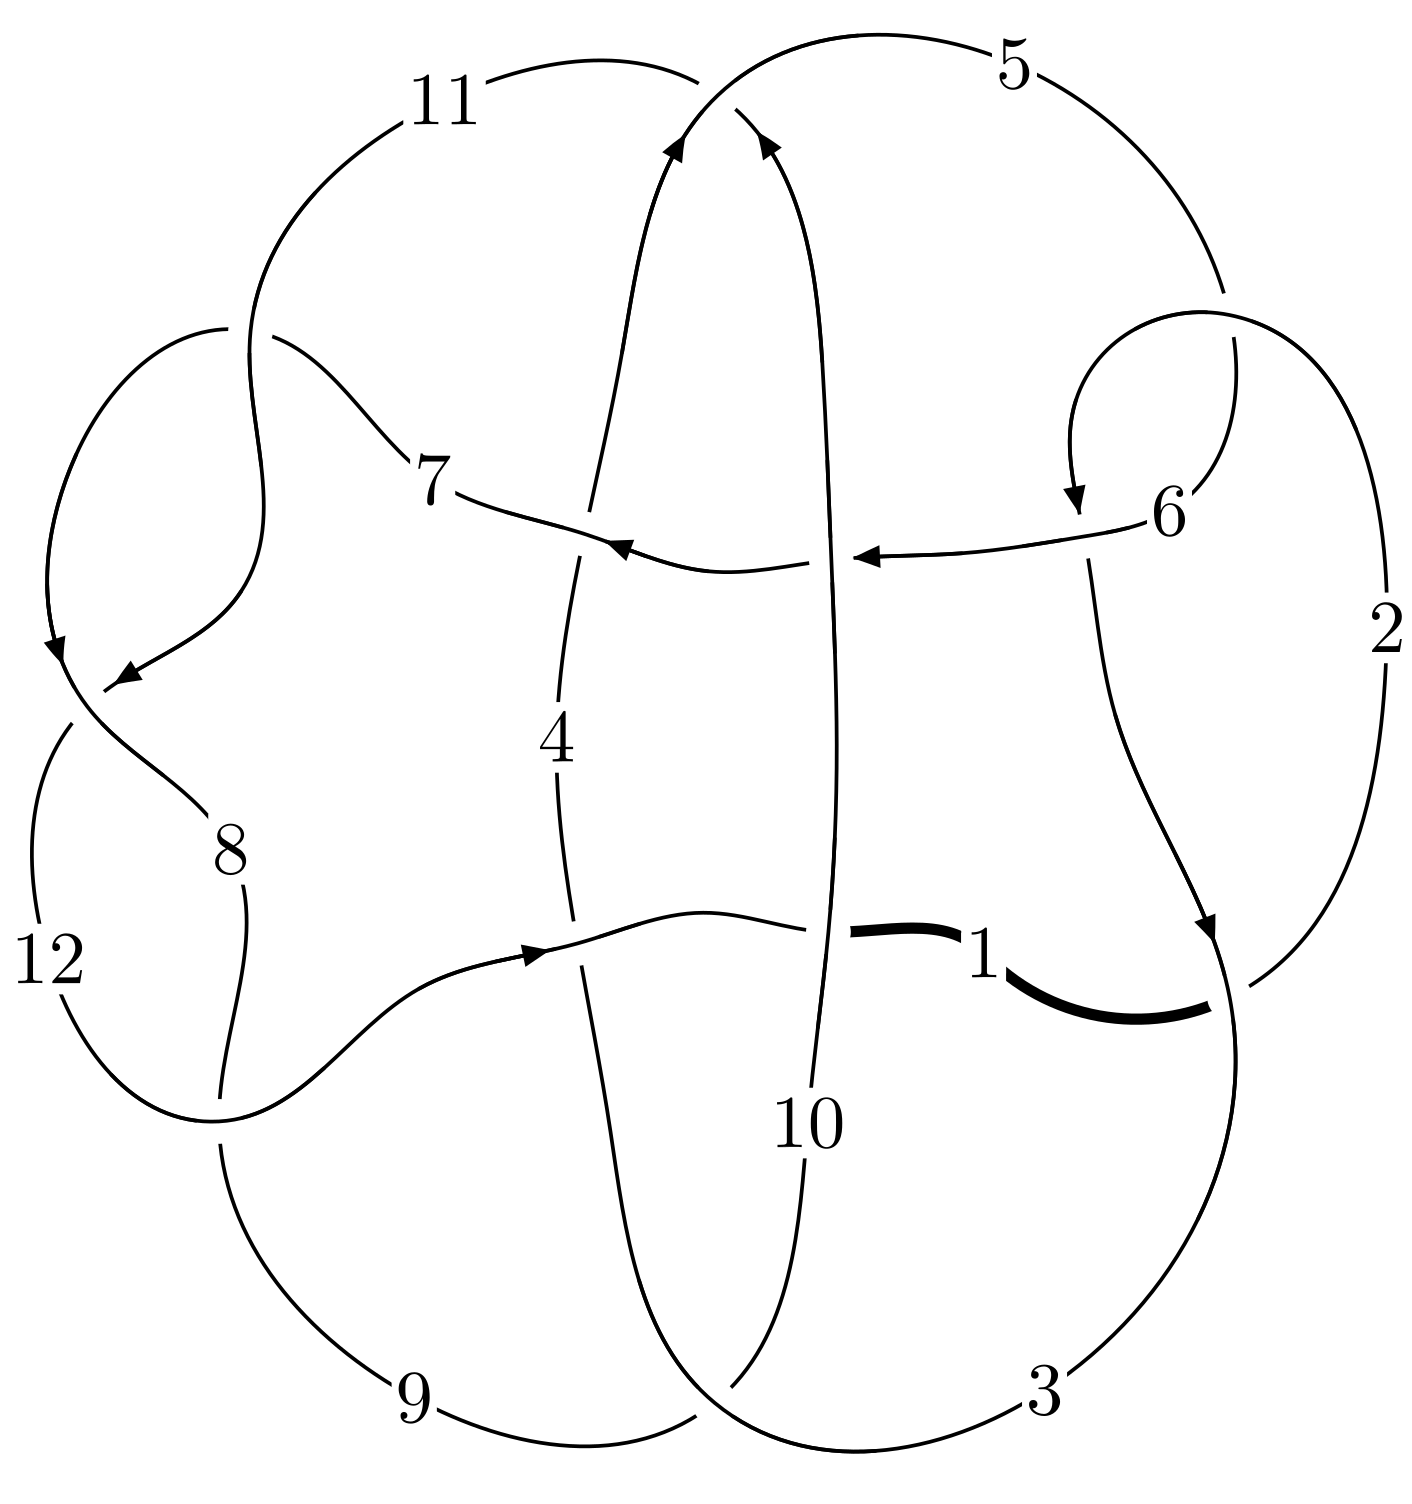
\includegraphics[width=112pt]{../../../GIT/diagram.site/Diagrams/png/2529_12n_0440.png}\\
\ \ \ A knot diagram\footnotemark}&
\allowdisplaybreaks
\textbf{Linearized knot diagam} \\
\cline{2-2}
 &
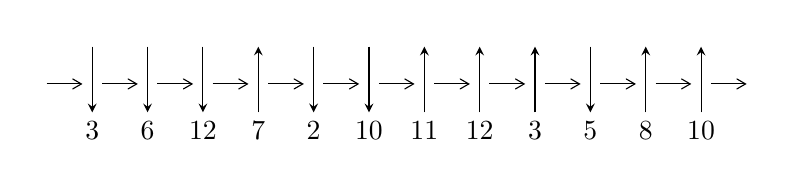
\begin{tikzpicture}[x=20pt, y=17pt]
	% nodes
	\node (C0) at (0, 0) {};
	\node (C1) at (1, 0) {};
	\node (C1U) at (1, +1) {};
	\node (C1D) at (1, -1) {3};

	\node (C2) at (2, 0) {};
	\node (C2U) at (2, +1) {};
	\node (C2D) at (2, -1) {6};

	\node (C3) at (3, 0) {};
	\node (C3U) at (3, +1) {};
	\node (C3D) at (3, -1) {12};

	\node (C4) at (4, 0) {};
	\node (C4U) at (4, +1) {};
	\node (C4D) at (4, -1) {7};

	\node (C5) at (5, 0) {};
	\node (C5U) at (5, +1) {};
	\node (C5D) at (5, -1) {2};

	\node (C6) at (6, 0) {};
	\node (C6U) at (6, +1) {};
	\node (C6D) at (6, -1) {10};

	\node (C7) at (7, 0) {};
	\node (C7U) at (7, +1) {};
	\node (C7D) at (7, -1) {11};

	\node (C8) at (8, 0) {};
	\node (C8U) at (8, +1) {};
	\node (C8D) at (8, -1) {12};

	\node (C9) at (9, 0) {};
	\node (C9U) at (9, +1) {};
	\node (C9D) at (9, -1) {3};

	\node (C10) at (10, 0) {};
	\node (C10U) at (10, +1) {};
	\node (C10D) at (10, -1) {5};

	\node (C11) at (11, 0) {};
	\node (C11U) at (11, +1) {};
	\node (C11D) at (11, -1) {8};

	\node (C12) at (12, 0) {};
	\node (C12U) at (12, +1) {};
	\node (C12D) at (12, -1) {10};
	\node (C13) at (13, 0) {};

	% arrows
	\draw[->,>={angle 60}]
	(C0) edge (C1) (C1) edge (C2) (C2) edge (C3) (C3) edge (C4) (C4) edge (C5) (C5) edge (C6) (C6) edge (C7) (C7) edge (C8) (C8) edge (C9) (C9) edge (C10) (C10) edge (C11) (C11) edge (C12) (C12) edge (C13) ;	\draw[->,>=stealth]
	(C1U) edge (C1D) (C2U) edge (C2D) (C3U) edge (C3D) (C4D) edge (C4U) (C5U) edge (C5D) (C6U) edge (C6D) (C7D) edge (C7U) (C8D) edge (C8U) (C9D) edge (C9U) (C10U) edge (C10D) (C11D) edge (C11U) (C12D) edge (C12U) ;
	\end{tikzpicture} \\
\hhline{~~} \\& 
\textbf{Solving Sequence} \\ \cline{2-2} 
 &
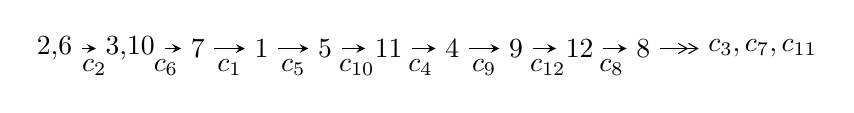
\begin{tikzpicture}[x=23pt, y=7pt]
	% node
	\node (A0) at (-1/8, 0) {2,6};
	\node (A1) at (17/16, 0) {3,10};
	\node (A2) at (17/8, 0) {7};
	\node (A3) at (25/8, 0) {1};
	\node (A4) at (33/8, 0) {5};
	\node (A5) at (41/8, 0) {11};
	\node (A6) at (49/8, 0) {4};
	\node (A7) at (57/8, 0) {9};
	\node (A8) at (65/8, 0) {12};
	\node (A9) at (73/8, 0) {8};
	\node (C1) at (1/2, -1) {$c_{2}$};
	\node (C2) at (13/8, -1) {$c_{6}$};
	\node (C3) at (21/8, -1) {$c_{1}$};
	\node (C4) at (29/8, -1) {$c_{5}$};
	\node (C5) at (37/8, -1) {$c_{10}$};
	\node (C6) at (45/8, -1) {$c_{4}$};
	\node (C7) at (53/8, -1) {$c_{9}$};
	\node (C8) at (61/8, -1) {$c_{12}$};
	\node (C9) at (69/8, -1) {$c_{8}$};
	\node (A10) at (11, 0) {$c_{3},c_{7},c_{11}$};

	% edge
	\draw[->,>=stealth]	
	(A0) edge (A1) (A1) edge (A2) (A2) edge (A3) (A3) edge (A4) (A4) edge (A5) (A5) edge (A6) (A6) edge (A7) (A7) edge (A8) (A8) edge (A9) ;
	\draw[->>,>={angle 60}]	
	(A9) edge (A10);
\end{tikzpicture} \\ 

\end{tabular} \\

\footnotetext{
The image of knot diagram is generated by the software ``\textbf{Draw programme}" developed by Andrew Bartholomew(\url{http://www.layer8.co.uk/maths/draw/index.htm\#Running-draw}), where we modified some parts for our purpose(\url{https://github.com/CATsTAILs/LinksPainter}).
}\phantom \\ \newline 
\centering \textbf{Ideals for irreducible components\footnotemark of $X_{\text{par}}$} 
 
\begin{align*}
I^u_{1}&=\langle 
-238 u^{25}-929 u^{24}+\cdots+288 b-10325,\;-1220 u^{25}-4477 u^{24}+\cdots+2976 a-43144,\\
\phantom{I^u_{1}}&\phantom{= \langle  }u^{26}+4 u^{25}+\cdots+112 u+31\rangle \\
I^u_{2}&=\langle 
-3 u^7+u^6+2 u^5-2 u^4-7 u^3+3 u^2+2 b+3 u-3,\;-3 u^7+3 u^6+2 u^5-2 u^4-7 u^3+7 u^2+2 a+3 u-3,\\
\phantom{I^u_{2}}&\phantom{= \langle  }u^8- u^6+3 u^4-2 u^2+1\rangle \\
I^u_{3}&=\langle 
u^{11}+u^{10}-3 u^9- u^8+3 u^7- u^6+4 u^5+4 u^4-5 u^3+u^2+4 b-4 u,\\
\phantom{I^u_{3}}&\phantom{= \langle  }u^{10}+u^9-3 u^8-3 u^7+5 u^6+3 u^5-2 u^4+4 u^3- u^2+4 a-9 u+4,\\
\phantom{I^u_{3}}&\phantom{= \langle  }u^{12}-4 u^{10}+u^9+6 u^8-3 u^7+u^6+3 u^5-9 u^4-2 u^3+5 u^2+u+2\rangle \\
I^u_{4}&=\langle 
- a^2+b-2 a,\;a^3+2 a^2+a-1,\;u-1\rangle \\
I^u_{5}&=\langle 
b^2 a-2 a^2 b+a^3- b+2 a-1,\;u-1\rangle \\
\\
I^v_{1}&=\langle 
a,\;b^3+b+1,\;v-1\rangle \\
\end{align*}
\raggedright * 5 irreducible components of $\dim_{\mathbb{C}}=0$, with total 52 representations.\\
\raggedright * 1 irreducible components of $\dim_{\mathbb{C}}=1$ \\
\footnotetext{All coefficients of polynomials are rational numbers. But the coefficients are sometimes approximated in decimal forms when there is not enough margin.}
\newpage
\renewcommand{\arraystretch}{1}
\centering \section*{I. $I^u_{1}= \langle -238 u^{25}-929 u^{24}+\cdots+288 b-10325,\;-1220 u^{25}-4477 u^{24}+\cdots+2976 a-43144,\;u^{26}+4 u^{25}+\cdots+112 u+31 \rangle$}
\flushleft \textbf{(i) Arc colorings}\\
\begin{tabular}{m{7pt} m{180pt} m{7pt} m{180pt} }
\flushright $a_{2}=$&$\begin{pmatrix}1\\0\end{pmatrix}$ \\
\flushright $a_{6}=$&$\begin{pmatrix}0\\u\end{pmatrix}$ \\
\flushright $a_{3}=$&$\begin{pmatrix}1\\u^2\end{pmatrix}$ \\
\flushright $a_{10}=$&$\begin{pmatrix}0.409946 u^{25}+1.50437 u^{24}+\cdots+39.5783 u+14.4973\\0.826389 u^{25}+3.22569 u^{24}+\cdots+93.5139 u+35.8507\end{pmatrix}$ \\
\flushright $a_{7}=$&$\begin{pmatrix}0.353831 u^{25}+1.25907 u^{24}+\cdots+37.8982 u+14.2540\\0.291667 u^{25}+1.11458 u^{24}+\cdots+35.6354 u+14.5208\end{pmatrix}$ \\
\flushright $a_{1}=$&$\begin{pmatrix}- u^2+1\\- u^4\end{pmatrix}$ \\
\flushright $a_{5}=$&$\begin{pmatrix}u\\u\end{pmatrix}$ \\
\flushright $a_{11}=$&$\begin{pmatrix}1.13564 u^{25}+2.78909 u^{24}+\cdots+58.7102 u+16.2195\\1.55208 u^{25}+4.51042 u^{24}+\cdots+112.646 u+37.5729\end{pmatrix}$ \\
\flushright $a_{4}=$&$\begin{pmatrix}0.663306 u^{25}+1.65323 u^{24}+\cdots+36.2944 u+11.7278\\0.937500 u^{25}+2.37500 u^{24}+\cdots+54.1875 u+16.6875\end{pmatrix}$ \\
\flushright $a_{9}=$&$\begin{pmatrix}-0.833109 u^{25}-2.14841 u^{24}+\cdots-51.4773 u-17.1555\\-0.291667 u^{25}-0.739583 u^{24}+\cdots-15.7292 u-5.05208\end{pmatrix}$ \\
\flushright $a_{12}=$&$\begin{pmatrix}0.0413306 u^{25}+0.290323 u^{24}+\cdots+12.3044 u+6.87903\\-0.270833 u^{25}-0.572917 u^{24}+\cdots-9.11458 u-0.979167\end{pmatrix}$ \\
\flushright $a_{8}=$&$\begin{pmatrix}-0.573029 u^{25}-1.26434 u^{24}+\cdots-24.9541 u-7.52643\\-\frac{1}{2} u^{25}-\frac{11}{8} u^{24}+\cdots-\frac{65}{2} u-\frac{87}{8}\end{pmatrix}$\\&\end{tabular}
\flushleft \textbf{(ii) Obstruction class $= -1$}\\~\\
\flushleft \textbf{(iii) Cusp Shapes $= -\frac{323}{108} u^{25}-\frac{262}{27} u^{24}+\cdots-\frac{7238}{27} u-\frac{2566}{27}$}\\~\\
\newpage\renewcommand{\arraystretch}{1}
\flushleft \textbf{(iv) u-Polynomials at the component}\newline \\
\begin{tabular}{m{50pt}|m{274pt}}
Crossings & \hspace{64pt}u-Polynomials at each crossing \\
\hline $$\begin{aligned}c_{1}\end{aligned}$$&$\begin{aligned}
&u^{26}+14 u^{25}+\cdots+1446 u+961
\end{aligned}$\\
\hline $$\begin{aligned}c_{2},c_{5}\end{aligned}$$&$\begin{aligned}
&u^{26}-4 u^{25}+\cdots-112 u+31
\end{aligned}$\\
\hline $$\begin{aligned}c_{3}\end{aligned}$$&$\begin{aligned}
&2(2 u^{26}-10 u^{25}+\cdots+864 u+183)
\end{aligned}$\\
\hline $$\begin{aligned}c_{4}\end{aligned}$$&$\begin{aligned}
&2(2 u^{26}+6 u^{25}+\cdots+6 u+93)
\end{aligned}$\\
\hline $$\begin{aligned}c_{6}\end{aligned}$$&$\begin{aligned}
&2(2 u^{26}+6 u^{25}+\cdots+828 u+216)
\end{aligned}$\\
\hline $$\begin{aligned}c_{7},c_{8},c_{11}\end{aligned}$$&$\begin{aligned}
&u^{26}+4 u^{25}+\cdots+104 u+31
\end{aligned}$\\
\hline $$\begin{aligned}c_{9}\end{aligned}$$&$\begin{aligned}
&3(3 u^{26}+6 u^{25}+\cdots+28 u+8)
\end{aligned}$\\
\hline $$\begin{aligned}c_{10}\end{aligned}$$&$\begin{aligned}
&3(3 u^{26}+6 u^{25}+\cdots-28 u+8)
\end{aligned}$\\
\hline $$\begin{aligned}c_{12}\end{aligned}$$&$\begin{aligned}
&2(2 u^{26}+2 u^{25}+\cdots+552 u+264)
\end{aligned}$\\
\hline
\end{tabular}\\~\\
\newpage\renewcommand{\arraystretch}{1}
\flushleft \textbf{(v) Riley Polynomials at the component}\newline \\
\begin{tabular}{m{50pt}|m{274pt}}
Crossings & \hspace{64pt}Riley Polynomials at each crossing \\
\hline $$\begin{aligned}c_{1}\end{aligned}$$&$\begin{aligned}
&y^{26}-2 y^{25}+\cdots-2335010 y+923521
\end{aligned}$\\
\hline $$\begin{aligned}c_{2},c_{5}\end{aligned}$$&$\begin{aligned}
&y^{26}-14 y^{25}+\cdots-1446 y+961
\end{aligned}$\\
\hline $$\begin{aligned}c_{3}\end{aligned}$$&$\begin{aligned}
&4(4 y^{26}-152 y^{25}+\cdots+146544 y+33489)
\end{aligned}$\\
\hline $$\begin{aligned}c_{4}\end{aligned}$$&$\begin{aligned}
&4(4 y^{26}+56 y^{25}+\cdots+74364 y+8649)
\end{aligned}$\\
\hline $$\begin{aligned}c_{6}\end{aligned}$$&$\begin{aligned}
&4(4 y^{26}-88 y^{25}+\cdots-322704 y+46656)
\end{aligned}$\\
\hline $$\begin{aligned}c_{7},c_{8},c_{11}\end{aligned}$$&$\begin{aligned}
&y^{26}-22 y^{25}+\cdots+282 y+961
\end{aligned}$\\
\hline $$\begin{aligned}c_{9}\end{aligned}$$&$\begin{aligned}
&9(9 y^{26}+276 y^{25}+\cdots+4752 y+64)
\end{aligned}$\\
\hline $$\begin{aligned}c_{10}\end{aligned}$$&$\begin{aligned}
&9(9 y^{26}+60 y^{25}+\cdots+400 y+64)
\end{aligned}$\\
\hline $$\begin{aligned}c_{12}\end{aligned}$$&$\begin{aligned}
&4(4 y^{26}+184 y^{25}+\cdots+708000 y+69696)
\end{aligned}$\\
\hline
\end{tabular}\\~\\
\newpage\flushleft \textbf{(vi) Complex Volumes and Cusp Shapes}
$$\begin{array}{c|c|c}  
\text{Solutions to }I^u_{1}& \I (\text{vol} + \sqrt{-1}CS) & \text{Cusp shape}\\
 \hline 
\begin{aligned}
u &= \phantom{-}0.207245 + 0.967760 I \\
a &= -0.149721 + 1.284220 I \\
b &= -0.516236 + 0.281803 I\end{aligned}
 & -3.60172 - 2.61761 I & -0.26262 + 1.62312 I \\ \hline\begin{aligned}
u &= \phantom{-}0.207245 - 0.967760 I \\
a &= -0.149721 - 1.284220 I \\
b &= -0.516236 - 0.281803 I\end{aligned}
 & -3.60172 + 2.61761 I & -0.26262 - 1.62312 I \\ \hline\begin{aligned}
u &= \phantom{-}0.820953 + 0.396871 I \\
a &= -0.464795 + 0.712990 I \\
b &= -0.578506 + 0.981502 I\end{aligned}
 & -1.82983 - 1.27994 I & -6.43006 + 3.42409 I \\ \hline\begin{aligned}
u &= \phantom{-}0.820953 - 0.396871 I \\
a &= -0.464795 - 0.712990 I \\
b &= -0.578506 - 0.981502 I\end{aligned}
 & -1.82983 + 1.27994 I & -6.43006 - 3.42409 I \\ \hline\begin{aligned}
u &= \phantom{-}0.093519 + 1.101170 I \\
a &= \phantom{-}0.479969 + 1.064420 I \\
b &= -0.492737 + 0.320156 I\end{aligned}
 & -1.83826 + 8.69089 I & \phantom{-}1.85327 - 5.19152 I \\ \hline\begin{aligned}
u &= \phantom{-}0.093519 - 1.101170 I \\
a &= \phantom{-}0.479969 - 1.064420 I \\
b &= -0.492737 - 0.320156 I\end{aligned}
 & -1.83826 - 8.69089 I & \phantom{-}1.85327 + 5.19152 I \\ \hline\begin{aligned}
u &= -0.875136 + 0.787433 I \\
a &= \phantom{-}0.012821 + 0.379761 I \\
b &= \phantom{-}0.682772 - 0.320729 I\end{aligned}
 & \phantom{-}8.20037 + 2.96512 I & \phantom{-}10.04842 - 2.30654 I \\ \hline\begin{aligned}
u &= -0.875136 - 0.787433 I \\
a &= \phantom{-}0.012821 - 0.379761 I \\
b &= \phantom{-}0.682772 + 0.320729 I\end{aligned}
 & \phantom{-}8.20037 - 2.96512 I & \phantom{-}10.04842 + 2.30654 I \\ \hline\begin{aligned}
u &= -1.161750 + 0.364732 I \\
a &= \phantom{-}1.216800 - 0.327659 I \\
b &= \phantom{-}2.00120 - 0.76731 I\end{aligned}
 & -2.84479 + 4.92637 I & -3.47765 - 6.11098 I \\ \hline\begin{aligned}
u &= -1.161750 - 0.364732 I \\
a &= \phantom{-}1.216800 + 0.327659 I \\
b &= \phantom{-}2.00120 + 0.76731 I\end{aligned}
 & -2.84479 - 4.92637 I & -3.47765 + 6.11098 I\\
 \hline 
 \end{array}$$\newpage$$\begin{array}{c|c|c}  
\text{Solutions to }I^u_{1}& \I (\text{vol} + \sqrt{-1}CS) & \text{Cusp shape}\\
 \hline 
\begin{aligned}
u &= -0.641989 + 0.388321 I \\
a &= -0.17877 - 1.49759 I \\
b &= -0.812488 - 0.481122 I\end{aligned}
 & \phantom{-}1.35413 + 1.46610 I & \phantom{-}7.33690 - 4.93932 I \\ \hline\begin{aligned}
u &= -0.641989 - 0.388321 I \\
a &= -0.17877 + 1.49759 I \\
b &= -0.812488 + 0.481122 I\end{aligned}
 & \phantom{-}1.35413 - 1.46610 I & \phantom{-}7.33690 + 4.93932 I \\ \hline\begin{aligned}
u &= -0.128992 + 0.733180 I \\
a &= \phantom{-}1.24585 - 1.03021 I \\
b &= -0.0120395 - 0.0178498 I\end{aligned}
 & \phantom{-}4.13697 - 4.56838 I & \phantom{-}6.59727 + 4.70609 I \\ \hline\begin{aligned}
u &= -0.128992 - 0.733180 I \\
a &= \phantom{-}1.24585 + 1.03021 I \\
b &= -0.0120395 + 0.0178498 I\end{aligned}
 & \phantom{-}4.13697 + 4.56838 I & \phantom{-}6.59727 - 4.70609 I \\ \hline\begin{aligned}
u &= -1.183540 + 0.424868 I \\
a &= -1.024870 + 0.400952 I \\
b &= -2.00747 + 0.99437 I\end{aligned}
 & \phantom{-}0.97162 + 8.87300 I & \phantom{-}1.52140 - 7.94866 I \\ \hline\begin{aligned}
u &= -1.183540 - 0.424868 I \\
a &= -1.024870 - 0.400952 I \\
b &= -2.00747 - 0.99437 I\end{aligned}
 & \phantom{-}0.97162 - 8.87300 I & \phantom{-}1.52140 + 7.94866 I \\ \hline\begin{aligned}
u &= \phantom{-}0.940665 + 0.925328 I \\
a &= \phantom{-}0.514581 - 0.495678 I \\
b &= \phantom{-}0.869814 - 0.281626 I\end{aligned}
 & \phantom{-}5.50559 - 3.38335 I & -3.13078 + 3.33250 I \\ \hline\begin{aligned}
u &= \phantom{-}0.940665 - 0.925328 I \\
a &= \phantom{-}0.514581 + 0.495678 I \\
b &= \phantom{-}0.869814 + 0.281626 I\end{aligned}
 & \phantom{-}5.50559 + 3.38335 I & -3.13078 - 3.33250 I \\ \hline\begin{aligned}
u &= -1.342860 + 0.390773 I \\
a &= \phantom{-}0.978142 - 0.178240 I \\
b &= \phantom{-}1.78351 + 0.39115 I\end{aligned}
 & -8.47827 + 7.26693 I & -2.82019 - 4.69299 I \\ \hline\begin{aligned}
u &= -1.342860 - 0.390773 I \\
a &= \phantom{-}0.978142 + 0.178240 I \\
b &= \phantom{-}1.78351 - 0.39115 I\end{aligned}
 & -8.47827 - 7.26693 I & -2.82019 + 4.69299 I\\
 \hline 
 \end{array}$$\newpage$$\begin{array}{c|c|c}  
\text{Solutions to }I^u_{1}& \I (\text{vol} + \sqrt{-1}CS) & \text{Cusp shape}\\
 \hline 
\begin{aligned}
u &= \phantom{-}1.31172 + 0.58643 I \\
a &= \phantom{-}1.376260 - 0.051091 I \\
b &= \phantom{-}2.25303 + 0.42993 I\end{aligned}
 & -10.39120 - 9.04784 I & -3.60025 + 5.37589 I \\ \hline\begin{aligned}
u &= \phantom{-}1.31172 - 0.58643 I \\
a &= \phantom{-}1.376260 + 0.051091 I \\
b &= \phantom{-}2.25303 - 0.42993 I\end{aligned}
 & -10.39120 + 9.04784 I & -3.60025 - 5.37589 I \\ \hline\begin{aligned}
u &= -1.37849 + 0.40779 I \\
a &= -0.815957 + 0.087138 I \\
b &= -1.41656 - 0.61555 I\end{aligned}
 & -11.75740 + 1.91795 I & -5.35471 - 0.48729 I \\ \hline\begin{aligned}
u &= -1.37849 - 0.40779 I \\
a &= -0.815957 - 0.087138 I \\
b &= -1.41656 + 0.61555 I\end{aligned}
 & -11.75740 - 1.91795 I & -5.35471 + 0.48729 I \\ \hline\begin{aligned}
u &= \phantom{-}1.33866 + 0.56921 I \\
a &= -1.399980 - 0.153122 I \\
b &= -2.25429 - 0.76615 I\end{aligned}
 & -5.7462 - 14.6212 I & -0.28099 + 7.59450 I \\ \hline\begin{aligned}
u &= \phantom{-}1.33866 - 0.56921 I \\
a &= -1.399980 + 0.153122 I \\
b &= -2.25429 + 0.76615 I\end{aligned}
 & -5.7462 + 14.6212 I & -0.28099 - 7.59450 I\\
 \hline 
 \end{array}$$\newpage\newpage\renewcommand{\arraystretch}{1}
\centering \section*{II. $I^u_{2}= \langle -3 u^7+u^6+\cdots+2 b-3,\;-3 u^7+3 u^6+\cdots+2 a-3,\;u^8- u^6+3 u^4-2 u^2+1 \rangle$}
\flushleft \textbf{(i) Arc colorings}\\
\begin{tabular}{m{7pt} m{180pt} m{7pt} m{180pt} }
\flushright $a_{2}=$&$\begin{pmatrix}1\\0\end{pmatrix}$ \\
\flushright $a_{6}=$&$\begin{pmatrix}0\\u\end{pmatrix}$ \\
\flushright $a_{3}=$&$\begin{pmatrix}1\\u^2\end{pmatrix}$ \\
\flushright $a_{10}=$&$\begin{pmatrix}\frac{3}{2} u^7-\frac{3}{2} u^6+\cdots-\frac{3}{2} u+\frac{3}{2}\\\frac{3}{2} u^7-\frac{1}{2} u^6+\cdots-\frac{3}{2} u+\frac{3}{2}\end{pmatrix}$ \\
\flushright $a_{7}=$&$\begin{pmatrix}2 u^7-\frac{5}{2} u^6+u^4+5 u^3-\frac{13}{2} u^2+u+\frac{3}{2}\\\frac{5}{2} u^7-2 u^6+\cdots-\frac{1}{2} u+2\end{pmatrix}$ \\
\flushright $a_{1}=$&$\begin{pmatrix}- u^2+1\\- u^4\end{pmatrix}$ \\
\flushright $a_{5}=$&$\begin{pmatrix}u\\u\end{pmatrix}$ \\
\flushright $a_{11}=$&$\begin{pmatrix}\frac{3}{2} u^7-\frac{5}{2} u^6+\cdots-\frac{3}{2} u+\frac{5}{2}\\\frac{3}{2} u^7-\frac{3}{2} u^6+\cdots-\frac{3}{2} u+\frac{5}{2}\end{pmatrix}$ \\
\flushright $a_{4}=$&$\begin{pmatrix}-\frac{21}{4} u^7+\frac{15}{4} u^6+\cdots+\frac{27}{4} u-\frac{25}{4}\\-\frac{17}{4} u^7+\frac{9}{4} u^6+\cdots+\frac{27}{4} u-\frac{23}{4}\end{pmatrix}$ \\
\flushright $a_{9}=$&$\begin{pmatrix}\frac{1}{2} u^7-\frac{3}{2} u^6+\cdots-\frac{3}{2} u+\frac{3}{2}\\\frac{1}{2} u^7-\frac{1}{2} u^6+\cdots-\frac{1}{2} u+\frac{3}{2}\end{pmatrix}$ \\
\flushright $a_{12}=$&$\begin{pmatrix}\frac{3}{2} u^7-2 u^6+u^4+\frac{7}{2} u^3-6 u^2+\frac{1}{2} u+2\\2 u^7-\frac{3}{2} u^6- u^5+5 u^3-\frac{7}{2} u^2- u+\frac{3}{2}\end{pmatrix}$ \\
\flushright $a_{8}=$&$\begin{pmatrix}\frac{3}{2} u^7-2 u^6+u^4+\frac{5}{2} u^3-5 u^2+\frac{1}{2} u+1\\2 u^7-\frac{3}{2} u^6- u^5+u^4+4 u^3-\frac{7}{2} u^2+\frac{3}{2}\end{pmatrix}$\\&\end{tabular}
\flushleft \textbf{(ii) Obstruction class $= 1$}\\~\\
\flushleft \textbf{(iii) Cusp Shapes $= 4 u^6-4 u^4+12 u^2-4$}\\~\\
\newpage\renewcommand{\arraystretch}{1}
\flushleft \textbf{(iv) u-Polynomials at the component}\newline \\
\begin{tabular}{m{50pt}|m{274pt}}
Crossings & \hspace{64pt}u-Polynomials at each crossing \\
\hline $$\begin{aligned}c_{1}\end{aligned}$$&$\begin{aligned}
&(u^4- u^3+3 u^2-2 u+1)^2
\end{aligned}$\\
\hline $$\begin{aligned}c_{2},c_{5}\end{aligned}$$&$\begin{aligned}
&u^8- u^6+3 u^4-2 u^2+1
\end{aligned}$\\
\hline $$\begin{aligned}c_{3}\end{aligned}$$&$\begin{aligned}
&2(2 u^8+10 u^7+29 u^6+48 u^5+58 u^4+50 u^3+27 u^2+8 u+1)
\end{aligned}$\\
\hline $$\begin{aligned}c_{4}\end{aligned}$$&$\begin{aligned}
&2(2 u^8+6 u^7+17 u^6+24 u^5+30 u^4+16 u^3+11 u^2+2 u+1)
\end{aligned}$\\
\hline $$\begin{aligned}c_{6}\end{aligned}$$&$\begin{aligned}
&2(2 u^8-2 u^7-3 u^6+12 u^5+14 u^4+8 u^3+7 u^2+2 u+1)
\end{aligned}$\\
\hline $$\begin{aligned}c_{7},c_{8},c_{11}\end{aligned}$$&$\begin{aligned}
&u^8-5 u^6+7 u^4-2 u^2+1
\end{aligned}$\\
\hline $$\begin{aligned}c_{9},c_{10}\end{aligned}$$&$\begin{aligned}
&(u^2+1)^4
\end{aligned}$\\
\hline $$\begin{aligned}c_{12}\end{aligned}$$&$\begin{aligned}
&2(2 u^8-2 u^7-7 u^6+16 u^5+2 u^4-26 u^3+23 u^2-8 u+1)
\end{aligned}$\\
\hline
\end{tabular}\\~\\
\newpage\renewcommand{\arraystretch}{1}
\flushleft \textbf{(v) Riley Polynomials at the component}\newline \\
\begin{tabular}{m{50pt}|m{274pt}}
Crossings & \hspace{64pt}Riley Polynomials at each crossing \\
\hline $$\begin{aligned}c_{1}\end{aligned}$$&$\begin{aligned}
&(y^4+5 y^3+7 y^2+2 y+1)^2
\end{aligned}$\\
\hline $$\begin{aligned}c_{2},c_{5}\end{aligned}$$&$\begin{aligned}
&(y^4- y^3+3 y^2-2 y+1)^2
\end{aligned}$\\
\hline $$\begin{aligned}c_{3}\end{aligned}$$&$\begin{aligned}
&4(4 y^8+16 y^7+113 y^6+168 y^5-26 y^4-78 y^3+45 y^2-10 y+1)
\end{aligned}$\\
\hline $$\begin{aligned}c_{4}\end{aligned}$$&$\begin{aligned}
&4(4 y^8+32 y^7+\cdots+18 y+1)
\end{aligned}$\\
\hline $$\begin{aligned}c_{6}\end{aligned}$$&$\begin{aligned}
&4(4 y^8-16 y^7+113 y^6-168 y^5-26 y^4+78 y^3+45 y^2+10 y+1)
\end{aligned}$\\
\hline $$\begin{aligned}c_{7},c_{8},c_{11}\end{aligned}$$&$\begin{aligned}
&(y^4-5 y^3+7 y^2-2 y+1)^2
\end{aligned}$\\
\hline $$\begin{aligned}c_{9},c_{10}\end{aligned}$$&$\begin{aligned}
&(y+1)^8
\end{aligned}$\\
\hline $$\begin{aligned}c_{12}\end{aligned}$$&$\begin{aligned}
&4(4 y^8-32 y^7+\cdots-18 y+1)
\end{aligned}$\\
\hline
\end{tabular}\\~\\
\newpage\flushleft \textbf{(vi) Complex Volumes and Cusp Shapes}
$$\begin{array}{c|c|c}  
\text{Solutions to }I^u_{2}& \I (\text{vol} + \sqrt{-1}CS) & \text{Cusp shape}\\
 \hline 
\begin{aligned}
u &= \phantom{-}0.720342 + 0.351808 I \\
a &= -0.433324 - 0.562927 I \\
b &= \phantom{-}0.114099 + 0.557947 I\end{aligned}
 & -0.21101 - 1.41510 I & \phantom{-}0.17326 + 4.90874 I \\ \hline\begin{aligned}
u &= \phantom{-}0.720342 - 0.351808 I \\
a &= -0.433324 + 0.562927 I \\
b &= \phantom{-}0.114099 - 0.557947 I\end{aligned}
 & -0.21101 + 1.41510 I & \phantom{-}0.17326 - 4.90874 I \\ \hline\begin{aligned}
u &= -0.720342 + 0.351808 I \\
a &= \phantom{-}1.19439 + 2.50547 I \\
b &= \phantom{-}1.74182 + 1.38460 I\end{aligned}
 & -0.21101 + 1.41510 I & \phantom{-}0.17326 - 4.90874 I \\ \hline\begin{aligned}
u &= -0.720342 - 0.351808 I \\
a &= \phantom{-}1.19439 - 2.50547 I \\
b &= \phantom{-}1.74182 - 1.38460 I\end{aligned}
 & -0.21101 - 1.41510 I & \phantom{-}0.17326 + 4.90874 I \\ \hline\begin{aligned}
u &= \phantom{-}0.911292 + 0.851808 I \\
a &= \phantom{-}0.352886 + 0.149146 I \\
b &= -0.194538 - 0.436506 I\end{aligned}
 & \phantom{-}6.79074 - 3.16396 I & \phantom{-}3.82674 + 2.56480 I \\ \hline\begin{aligned}
u &= \phantom{-}0.911292 - 0.851808 I \\
a &= \phantom{-}0.352886 - 0.149146 I \\
b &= -0.194538 + 0.436506 I\end{aligned}
 & \phantom{-}6.79074 + 3.16396 I & \phantom{-}3.82674 - 2.56480 I \\ \hline\begin{aligned}
u &= -0.911292 + 0.851808 I \\
a &= -0.613954 - 0.706599 I \\
b &= -1.161380 - 0.120947 I\end{aligned}
 & \phantom{-}6.79074 + 3.16396 I & \phantom{-}3.82674 - 2.56480 I \\ \hline\begin{aligned}
u &= -0.911292 - 0.851808 I \\
a &= -0.613954 + 0.706599 I \\
b &= -1.161380 + 0.120947 I\end{aligned}
 & \phantom{-}6.79074 - 3.16396 I & \phantom{-}3.82674 + 2.56480 I\\
 \hline 
 \end{array}$$\newpage\newpage\renewcommand{\arraystretch}{1}
\centering \section*{III. $I^u_{3}= \langle u^{11}+u^{10}+\cdots+4 b-4 u,\;u^{10}+u^9+\cdots+4 a+4,\;u^{12}-4 u^{10}+\cdots+u+2 \rangle$}
\flushleft \textbf{(i) Arc colorings}\\
\begin{tabular}{m{7pt} m{180pt} m{7pt} m{180pt} }
\flushright $a_{2}=$&$\begin{pmatrix}1\\0\end{pmatrix}$ \\
\flushright $a_{6}=$&$\begin{pmatrix}0\\u\end{pmatrix}$ \\
\flushright $a_{3}=$&$\begin{pmatrix}1\\u^2\end{pmatrix}$ \\
\flushright $a_{10}=$&$\begin{pmatrix}-\frac{1}{4} u^{10}-\frac{1}{4} u^9+\cdots+\frac{9}{4} u-1\\-\frac{1}{4} u^{11}-\frac{1}{4} u^{10}+\cdots-\frac{1}{4} u^2+u\end{pmatrix}$ \\
\flushright $a_{7}=$&$\begin{pmatrix}-\frac{1}{4} u^{10}+\frac{5}{4} u^8+\cdots-\frac{1}{2} u-\frac{1}{2}\\-\frac{1}{4} u^9+\frac{1}{2} u^8+\cdots+\frac{5}{4} u+\frac{1}{2}\end{pmatrix}$ \\
\flushright $a_{1}=$&$\begin{pmatrix}- u^2+1\\- u^4\end{pmatrix}$ \\
\flushright $a_{5}=$&$\begin{pmatrix}u\\u\end{pmatrix}$ \\
\flushright $a_{11}=$&$\begin{pmatrix}-\frac{1}{4} u^9+\frac{3}{4} u^7+\cdots+\frac{7}{4} u-1\\-\frac{1}{4} u^{11}+\frac{3}{4} u^9+\cdots-\frac{3}{2} u^2+\frac{1}{2} u\end{pmatrix}$ \\
\flushright $a_{4}=$&$\begin{pmatrix}\frac{1}{2} u^{11}-\frac{1}{4} u^{10}+\cdots-\frac{1}{2} u+\frac{3}{2}\\\frac{1}{2} u^{11}- u^9+\cdots-\frac{1}{4} u+\frac{1}{2}\end{pmatrix}$ \\
\flushright $a_{9}=$&$\begin{pmatrix}-\frac{1}{4} u^{10}+\frac{3}{4} u^8+\cdots+\frac{3}{2} u-\frac{1}{2}\\-\frac{1}{4} u^{10}+\frac{3}{4} u^8+\cdots+\frac{1}{4} u^2+u\end{pmatrix}$ \\
\flushright $a_{12}=$&$\begin{pmatrix}-\frac{1}{4} u^9+\frac{1}{4} u^7+\cdots-\frac{5}{4} u+1\\-\frac{1}{2} u^9+u^7+\cdots+\frac{1}{2} u^2-\frac{1}{2} u\end{pmatrix}$ \\
\flushright $a_{8}=$&$\begin{pmatrix}\frac{1}{2} u^8- u^6+\cdots+\frac{1}{2} u-\frac{1}{2}\\\frac{1}{4} u^{10}-\frac{1}{4} u^8+\cdots+\frac{3}{4} u^2+u\end{pmatrix}$\\&\end{tabular}
\flushleft \textbf{(ii) Obstruction class $= -1$}\\~\\
\flushleft \textbf{(iii) Cusp Shapes $= -2 u^9+6 u^7-2 u^6-6 u^5+4 u^4-6 u^3-2 u^2+8 u+2$}\\~\\
\newpage\renewcommand{\arraystretch}{1}
\flushleft \textbf{(iv) u-Polynomials at the component}\newline \\
\begin{tabular}{m{50pt}|m{274pt}}
Crossings & \hspace{64pt}u-Polynomials at each crossing \\
\hline $$\begin{aligned}c_{1}\end{aligned}$$&$\begin{aligned}
&u^{12}+8 u^{11}+\cdots-19 u+4
\end{aligned}$\\
\hline $$\begin{aligned}c_{2},c_{5},c_{7}\\c_{8},c_{11}\end{aligned}$$&$\begin{aligned}
&u^{12}-4 u^{10}- u^9+6 u^8+3 u^7+u^6-3 u^5-9 u^4+2 u^3+5 u^2- u+2
\end{aligned}$\\
\hline $$\begin{aligned}c_{3}\end{aligned}$$&$\begin{aligned}
&2(2 u^{12}+2 u^{11}+\cdots-56 u+8)
\end{aligned}$\\
\hline $$\begin{aligned}c_{4}\end{aligned}$$&$\begin{aligned}
&2(2 u^{12}+10 u^{11}+\cdots+12 u+8)
\end{aligned}$\\
\hline $$\begin{aligned}c_{6}\end{aligned}$$&$\begin{aligned}
&2(2 u^{12}-2 u^{11}+\cdots+66 u+47)
\end{aligned}$\\
\hline $$\begin{aligned}c_{9}\end{aligned}$$&$\begin{aligned}
&(u^4- u^3+3 u^2-2 u+1)^3
\end{aligned}$\\
\hline $$\begin{aligned}c_{10}\end{aligned}$$&$\begin{aligned}
&(u^4- u^3+u^2+1)^3
\end{aligned}$\\
\hline $$\begin{aligned}c_{12}\end{aligned}$$&$\begin{aligned}
&2(2 u^{12}-6 u^{11}+\cdots-150 u+103)
\end{aligned}$\\
\hline
\end{tabular}\\~\\
\newpage\renewcommand{\arraystretch}{1}
\flushleft \textbf{(v) Riley Polynomials at the component}\newline \\
\begin{tabular}{m{50pt}|m{274pt}}
Crossings & \hspace{64pt}Riley Polynomials at each crossing \\
\hline $$\begin{aligned}c_{1}\end{aligned}$$&$\begin{aligned}
&y^{12}-8 y^{11}+\cdots-417 y+16
\end{aligned}$\\
\hline $$\begin{aligned}c_{2},c_{5},c_{7}\\c_{8},c_{11}\end{aligned}$$&$\begin{aligned}
&y^{12}-8 y^{11}+\cdots+19 y+4
\end{aligned}$\\
\hline $$\begin{aligned}c_{3}\end{aligned}$$&$\begin{aligned}
&4(4 y^{12}-88 y^{11}+\cdots+2080 y+64)
\end{aligned}$\\
\hline $$\begin{aligned}c_{4}\end{aligned}$$&$\begin{aligned}
&4(4 y^{12}+16 y^{11}+\cdots+688 y+64)
\end{aligned}$\\
\hline $$\begin{aligned}c_{6}\end{aligned}$$&$\begin{aligned}
&4(4 y^{12}-56 y^{11}+\cdots-4168 y+2209)
\end{aligned}$\\
\hline $$\begin{aligned}c_{9}\end{aligned}$$&$\begin{aligned}
&(y^4+5 y^3+7 y^2+2 y+1)^3
\end{aligned}$\\
\hline $$\begin{aligned}c_{10}\end{aligned}$$&$\begin{aligned}
&(y^4+y^3+3 y^2+2 y+1)^3
\end{aligned}$\\
\hline $$\begin{aligned}c_{12}\end{aligned}$$&$\begin{aligned}
&4(4 y^{12}+80 y^{11}+\cdots+116344 y+10609)
\end{aligned}$\\
\hline
\end{tabular}\\~\\
\newpage\flushleft \textbf{(vi) Complex Volumes and Cusp Shapes}
$$\begin{array}{c|c|c}  
\text{Solutions to }I^u_{3}& \I (\text{vol} + \sqrt{-1}CS) & \text{Cusp shape}\\
 \hline 
\begin{aligned}
u &= \phantom{-}0.152073 + 1.050790 I \\
a &= -0.216032 - 1.219810 I \\
b &= \phantom{-}0.518508 - 0.302871 I\end{aligned}
 & -6.79074 + 3.16396 I & -1.82674 - 2.56480 I \\ \hline\begin{aligned}
u &= \phantom{-}0.152073 - 1.050790 I \\
a &= -0.216032 + 1.219810 I \\
b &= \phantom{-}0.518508 + 0.302871 I\end{aligned}
 & -6.79074 - 3.16396 I & -1.82674 + 2.56480 I \\ \hline\begin{aligned}
u &= -1.043920 + 0.280279 I \\
a &= -1.82414 - 0.12229 I \\
b &= -2.31130 + 0.43695 I\end{aligned}
 & \phantom{-}0.21101 + 1.41510 I & \phantom{-}1.82674 - 4.90874 I \\ \hline\begin{aligned}
u &= -1.043920 - 0.280279 I \\
a &= -1.82414 + 0.12229 I \\
b &= -2.31130 - 0.43695 I\end{aligned}
 & \phantom{-}0.21101 - 1.41510 I & \phantom{-}1.82674 + 4.90874 I \\ \hline\begin{aligned}
u &= \phantom{-}1.131290 + 0.219998 I \\
a &= \phantom{-}0.169450 - 1.077300 I \\
b &= \phantom{-}0.34978 - 1.74911 I\end{aligned}
 & \phantom{-}0.21101 + 1.41510 I & \phantom{-}1.82674 - 4.90874 I \\ \hline\begin{aligned}
u &= \phantom{-}1.131290 - 0.219998 I \\
a &= \phantom{-}0.169450 + 1.077300 I \\
b &= \phantom{-}0.34978 + 1.74911 I\end{aligned}
 & \phantom{-}0.21101 - 1.41510 I & \phantom{-}1.82674 + 4.90874 I \\ \hline\begin{aligned}
u &= \phantom{-}1.272550 + 0.614267 I \\
a &= -1.238380 + 0.267755 I \\
b &= -2.06161 - 0.05098 I\end{aligned}
 & -6.79074 - 3.16396 I & -1.82674 + 2.56480 I \\ \hline\begin{aligned}
u &= \phantom{-}1.272550 - 0.614267 I \\
a &= -1.238380 - 0.267755 I \\
b &= -2.06161 + 0.05098 I\end{aligned}
 & -6.79074 + 3.16396 I & -1.82674 - 2.56480 I \\ \hline\begin{aligned}
u &= -1.42462 + 0.43653 I \\
a &= \phantom{-}0.618232 - 0.037304 I \\
b &= \phantom{-}0.985647 + 0.714952 I\end{aligned}
 & -6.79074 - 3.16396 I & -1.82674 + 2.56480 I \\ \hline\begin{aligned}
u &= -1.42462 - 0.43653 I \\
a &= \phantom{-}0.618232 + 0.037304 I \\
b &= \phantom{-}0.985647 - 0.714952 I\end{aligned}
 & -6.79074 + 3.16396 I & -1.82674 - 2.56480 I\\
 \hline 
 \end{array}$$\newpage$$\begin{array}{c|c|c}  
\text{Solutions to }I^u_{3}& \I (\text{vol} + \sqrt{-1}CS) & \text{Cusp shape}\\
 \hline 
\begin{aligned}
u &= -0.087368 + 0.500278 I \\
a &= -1.25913 + 1.24198 I \\
b &= \phantom{-}0.018967 + 0.315552 I\end{aligned}
 & \phantom{-}0.21101 - 1.41510 I & \phantom{-}1.82674 + 4.90874 I \\ \hline\begin{aligned}
u &= -0.087368 - 0.500278 I \\
a &= -1.25913 - 1.24198 I \\
b &= \phantom{-}0.018967 - 0.315552 I\end{aligned}
 & \phantom{-}0.21101 + 1.41510 I & \phantom{-}1.82674 - 4.90874 I\\
 \hline 
 \end{array}$$\newpage\newpage\renewcommand{\arraystretch}{1}
\centering \section*{IV. $I^u_{4}= \langle - a^2+b-2 a,\;a^3+2 a^2+a-1,\;u-1 \rangle$}
\flushleft \textbf{(i) Arc colorings}\\
\begin{tabular}{m{7pt} m{180pt} m{7pt} m{180pt} }
\flushright $a_{2}=$&$\begin{pmatrix}1\\0\end{pmatrix}$ \\
\flushright $a_{6}=$&$\begin{pmatrix}0\\1\end{pmatrix}$ \\
\flushright $a_{3}=$&$\begin{pmatrix}1\\1\end{pmatrix}$ \\
\flushright $a_{10}=$&$\begin{pmatrix}a\\a^2+2 a\end{pmatrix}$ \\
\flushright $a_{7}=$&$\begin{pmatrix}- a^2\\a\end{pmatrix}$ \\
\flushright $a_{1}=$&$\begin{pmatrix}0\\-1\end{pmatrix}$ \\
\flushright $a_{5}=$&$\begin{pmatrix}1\\1\end{pmatrix}$ \\
\flushright $a_{11}=$&$\begin{pmatrix}- a^2\\a\end{pmatrix}$ \\
\flushright $a_{4}=$&$\begin{pmatrix}- a^2-2 a+2\\- a^2- a+2\end{pmatrix}$ \\
\flushright $a_{9}=$&$\begin{pmatrix}- a^2\\a\end{pmatrix}$ \\
\flushright $a_{12}=$&$\begin{pmatrix}a^2\\- a\end{pmatrix}$ \\
\flushright $a_{8}=$&$\begin{pmatrix}- a^2\\a\end{pmatrix}$\\&\end{tabular}
\flushleft \textbf{(ii) Obstruction class $= -1$}\\~\\
\flushleft \textbf{(iii) Cusp Shapes $= -6$}\\~\\
\newpage\renewcommand{\arraystretch}{1}
\flushleft \textbf{(iv) u-Polynomials at the component}\newline \\
\begin{tabular}{m{50pt}|m{274pt}}
Crossings & \hspace{64pt}u-Polynomials at each crossing \\
\hline $$\begin{aligned}c_{1},c_{2},c_{5}\end{aligned}$$&$\begin{aligned}
&(u+1)^3
\end{aligned}$\\
\hline $$\begin{aligned}c_{3},c_{4},c_{9}\\c_{10}\end{aligned}$$&$\begin{aligned}
&u^3+u+1
\end{aligned}$\\
\hline $$\begin{aligned}c_{6}\end{aligned}$$&$\begin{aligned}
&u^3+2 u^2+u-1
\end{aligned}$\\
\hline $$\begin{aligned}c_{7},c_{8},c_{11}\end{aligned}$$&$\begin{aligned}
&u^3
\end{aligned}$\\
\hline $$\begin{aligned}c_{12}\end{aligned}$$&$\begin{aligned}
&u^3-2 u^2+u+1
\end{aligned}$\\
\hline
\end{tabular}\\~\\
\newpage\renewcommand{\arraystretch}{1}
\flushleft \textbf{(v) Riley Polynomials at the component}\newline \\
\begin{tabular}{m{50pt}|m{274pt}}
Crossings & \hspace{64pt}Riley Polynomials at each crossing \\
\hline $$\begin{aligned}c_{1},c_{2},c_{5}\end{aligned}$$&$\begin{aligned}
&(y-1)^3
\end{aligned}$\\
\hline $$\begin{aligned}c_{3},c_{4},c_{9}\\c_{10}\end{aligned}$$&$\begin{aligned}
&y^3+2 y^2+y-1
\end{aligned}$\\
\hline $$\begin{aligned}c_{6},c_{12}\end{aligned}$$&$\begin{aligned}
&y^3-2 y^2+5 y-1
\end{aligned}$\\
\hline $$\begin{aligned}c_{7},c_{8},c_{11}\end{aligned}$$&$\begin{aligned}
&y^3
\end{aligned}$\\
\hline
\end{tabular}\\~\\
\newpage\flushleft \textbf{(vi) Complex Volumes and Cusp Shapes}
$$\begin{array}{c|c|c}  
\text{Solutions to }I^u_{4}& \I (\text{vol} + \sqrt{-1}CS) & \text{Cusp shape}\\
 \hline 
\begin{aligned}
u &= \phantom{-}1.00000\phantom{ +0.000000I} \\
a &= -1.23279 + 0.79255 I \\
b &= -1.57395 - 0.36899 I\end{aligned}
 & -1.64493\phantom{ +0.000000I} & -6.00000\phantom{ +0.000000I} \\ \hline\begin{aligned}
u &= \phantom{-}1.00000\phantom{ +0.000000I} \\
a &= -1.23279 - 0.79255 I \\
b &= -1.57395 + 0.36899 I\end{aligned}
 & -1.64493\phantom{ +0.000000I} & -6.00000\phantom{ +0.000000I} \\ \hline\begin{aligned}
u &= \phantom{-}1.00000\phantom{ +0.000000I} \\
a &= \phantom{-}0.465571\phantom{ +0.000000I} \\
b &= \phantom{-}1.14790\phantom{ +0.000000I}\end{aligned}
 & -1.64493\phantom{ +0.000000I} & -6.00000\phantom{ +0.000000I}\\
 \hline 
 \end{array}$$\newpage\newpage\renewcommand{\arraystretch}{1}
\centering \section*{V. $I^u_{5}= \langle b^2 a-2 a^2 b+a^3- b+2 a-1,\;u-1 \rangle$}
\flushleft \textbf{(i) Arc colorings}\\
\begin{tabular}{m{7pt} m{180pt} m{7pt} m{180pt} }
\flushright $a_{2}=$&$\begin{pmatrix}1\\0\end{pmatrix}$ \\
\flushright $a_{6}=$&$\begin{pmatrix}0\\1\end{pmatrix}$ \\
\flushright $a_{3}=$&$\begin{pmatrix}1\\1\end{pmatrix}$ \\
\flushright $a_{10}=$&$\begin{pmatrix}a\\b\end{pmatrix}$ \\
\flushright $a_{7}=$&$\begin{pmatrix}- a^2\\- b a+1\end{pmatrix}$ \\
\flushright $a_{1}=$&$\begin{pmatrix}0\\-1\end{pmatrix}$ \\
\flushright $a_{5}=$&$\begin{pmatrix}1\\1\end{pmatrix}$ \\
\flushright $a_{11}=$&$\begin{pmatrix}- b+2 a\\a\end{pmatrix}$ \\
\flushright $a_{4}=$&$\begin{pmatrix}a^3 b- a^4- a^2+1\\a^3 b- a^4- b a- a^2+a+2\end{pmatrix}$ \\
\flushright $a_{9}=$&$\begin{pmatrix}- b+2 a\\a\end{pmatrix}$ \\
\flushright $a_{12}=$&$\begin{pmatrix}a^2\\b a-1\end{pmatrix}$ \\
\flushright $a_{8}=$&$\begin{pmatrix}- a^2- b+2 a\\- b a+a+1\end{pmatrix}$\\&\end{tabular}
\flushleft \textbf{(ii) Obstruction class $= 1$}\\~\\
\flushleft \textbf{(iii) Cusp Shapes $= 0$}\\~\\
\flushleft \textbf{(iv) u-Polynomials at the component} : It cannot be defined for a positive dimension component.\\~\\
\flushleft \textbf{(v) Riley Polynomials at the component} : It cannot be defined for a positive dimension component.\\~\\
\newpage\flushleft \textbf{(iv) Complex Volumes and Cusp Shapes}
$$\begin{array}{c|c|c} 
\text{Solution to }I^u_{5}& \I (\text{vol} + \sqrt{-1}CS) & \text{Cusp shape}\\
 \hline 
\begin{aligned}
u &= \cdots \\
a &= \cdots \\
b &= \cdots\end{aligned}
 & \phantom{-0.000000 } 0 & \phantom{-0.000000 } 0\\
 \hline 
 \end{array}
$$\newpage\renewcommand{\arraystretch}{1}
\centering \section*{VI. $I^v_{1}= \langle a,\;b^3+b+1,\;v-1 \rangle$}
\flushleft \textbf{(i) Arc colorings}\\
\begin{tabular}{m{7pt} m{180pt} m{7pt} m{180pt} }
\flushright $a_{2}=$&$\begin{pmatrix}1\\0\end{pmatrix}$ \\
\flushright $a_{6}=$&$\begin{pmatrix}1\\0\end{pmatrix}$ \\
\flushright $a_{3}=$&$\begin{pmatrix}1\\0\end{pmatrix}$ \\
\flushright $a_{10}=$&$\begin{pmatrix}0\\b\end{pmatrix}$ \\
\flushright $a_{7}=$&$\begin{pmatrix}1\\b^2\end{pmatrix}$ \\
\flushright $a_{1}=$&$\begin{pmatrix}1\\0\end{pmatrix}$ \\
\flushright $a_{5}=$&$\begin{pmatrix}1\\0\end{pmatrix}$ \\
\flushright $a_{11}=$&$\begin{pmatrix}- b\\b\end{pmatrix}$ \\
\flushright $a_{4}=$&$\begin{pmatrix}b^2+1\\- b^2- b\end{pmatrix}$ \\
\flushright $a_{9}=$&$\begin{pmatrix}- b\\b\end{pmatrix}$ \\
\flushright $a_{12}=$&$\begin{pmatrix}1\\b^2\end{pmatrix}$ \\
\flushright $a_{8}=$&$\begin{pmatrix}- b+1\\b^2+b\end{pmatrix}$\\&\end{tabular}
\flushleft \textbf{(ii) Obstruction class $= -1$}\\~\\
\flushleft \textbf{(iii) Cusp Shapes $= 6$}\\~\\
\newpage\renewcommand{\arraystretch}{1}
\flushleft \textbf{(iv) u-Polynomials at the component}\newline \\
\begin{tabular}{m{50pt}|m{274pt}}
Crossings & \hspace{64pt}u-Polynomials at each crossing \\
\hline $$\begin{aligned}c_{1},c_{2},c_{5}\end{aligned}$$&$\begin{aligned}
&u^3
\end{aligned}$\\
\hline $$\begin{aligned}c_{3}\end{aligned}$$&$\begin{aligned}
&u^3+2 u^2+u-1
\end{aligned}$\\
\hline $$\begin{aligned}c_{4}\end{aligned}$$&$\begin{aligned}
&u^3-2 u^2+u+1
\end{aligned}$\\
\hline $$\begin{aligned}c_{6},c_{9},c_{10}\\c_{12}\end{aligned}$$&$\begin{aligned}
&u^3+u-1
\end{aligned}$\\
\hline $$\begin{aligned}c_{7},c_{8},c_{11}\end{aligned}$$&$\begin{aligned}
&(u-1)^3
\end{aligned}$\\
\hline
\end{tabular}\\~\\
\newpage\renewcommand{\arraystretch}{1}
\flushleft \textbf{(v) Riley Polynomials at the component}\newline \\
\begin{tabular}{m{50pt}|m{274pt}}
Crossings & \hspace{64pt}Riley Polynomials at each crossing \\
\hline $$\begin{aligned}c_{1},c_{2},c_{5}\end{aligned}$$&$\begin{aligned}
&y^3
\end{aligned}$\\
\hline $$\begin{aligned}c_{3},c_{4}\end{aligned}$$&$\begin{aligned}
&y^3-2 y^2+5 y-1
\end{aligned}$\\
\hline $$\begin{aligned}c_{6},c_{9},c_{10}\\c_{12}\end{aligned}$$&$\begin{aligned}
&y^3+2 y^2+y-1
\end{aligned}$\\
\hline $$\begin{aligned}c_{7},c_{8},c_{11}\end{aligned}$$&$\begin{aligned}
&(y-1)^3
\end{aligned}$\\
\hline
\end{tabular}\\~\\
\newpage\flushleft \textbf{(vi) Complex Volumes and Cusp Shapes}
$$\begin{array}{c|c|c}  
\text{Solutions to }I^v_{1}& \I (\text{vol} + \sqrt{-1}CS) & \text{Cusp shape}\\
 \hline 
\begin{aligned}
v &= \phantom{-}1.00000\phantom{ +0.000000I} \\
a &= \phantom{-0.000000 } 0 \\
b &= \phantom{-}0.341164 + 1.161540 I\end{aligned}
 & \phantom{-}1.64493\phantom{ +0.000000I} & \phantom{-}6.00000\phantom{ +0.000000I} \\ \hline\begin{aligned}
v &= \phantom{-}1.00000\phantom{ +0.000000I} \\
a &= \phantom{-0.000000 } 0 \\
b &= \phantom{-}0.341164 - 1.161540 I\end{aligned}
 & \phantom{-}1.64493\phantom{ +0.000000I} & \phantom{-}6.00000\phantom{ +0.000000I} \\ \hline\begin{aligned}
v &= \phantom{-}1.00000\phantom{ +0.000000I} \\
a &= \phantom{-0.000000 } 0 \\
b &= -0.682328\phantom{ +0.000000I}\end{aligned}
 & \phantom{-}1.64493\phantom{ +0.000000I} & \phantom{-}6.00000\phantom{ +0.000000I}\\
 \hline 
 \end{array}$$\newpage
\newpage\renewcommand{\arraystretch}{1}
\centering \section*{ VII. u-Polynomials}
\begin{tabular}{m{50pt}|m{274pt}}
Crossings & \hspace{64pt}u-Polynomials at each crossing \\
\hline $$\begin{aligned}c_{1}\end{aligned}$$&$\begin{aligned}
&u^3(u+1)^3(u^4- u^3+\cdots-2 u+1)^{2}(u^{12}+8 u^{11}+\cdots-19 u+4)\\
&\cdot(u^{26}+14 u^{25}+\cdots+1446 u+961)
\end{aligned}$\\
\hline $$\begin{aligned}c_{2},c_{5}\end{aligned}$$&$\begin{aligned}
&u^3(u+1)^3(u^8- u^6+3 u^4-2 u^2+1)\\
&\cdot(u^{12}-4 u^{10}- u^9+6 u^8+3 u^7+u^6-3 u^5-9 u^4+2 u^3+5 u^2- u+2)\\
&\cdot(u^{26}-4 u^{25}+\cdots-112 u+31)
\end{aligned}$\\
\hline $$\begin{aligned}c_{3}\end{aligned}$$&$\begin{aligned}
&8(u^3+u+1)(u^3+2 u^2+u-1)\\
&\cdot(2 u^8+10 u^7+29 u^6+48 u^5+58 u^4+50 u^3+27 u^2+8 u+1)\\
&\cdot(2 u^{12}+2 u^{11}+\cdots-56 u+8)(2 u^{26}-10 u^{25}+\cdots+864 u+183)
\end{aligned}$\\
\hline $$\begin{aligned}c_{4}\end{aligned}$$&$\begin{aligned}
&8(u^3+u+1)(u^3-2 u^2+u+1)\\
&\cdot(2 u^8+6 u^7+17 u^6+24 u^5+30 u^4+16 u^3+11 u^2+2 u+1)\\
&\cdot(2 u^{12}+10 u^{11}+\cdots+12 u+8)(2 u^{26}+6 u^{25}+\cdots+6 u+93)
\end{aligned}$\\
\hline $$\begin{aligned}c_{6}\end{aligned}$$&$\begin{aligned}
&8(u^3+u-1)(u^3+2 u^2+u-1)\\
&\cdot(2 u^8-2 u^7-3 u^6+12 u^5+14 u^4+8 u^3+7 u^2+2 u+1)\\
&\cdot(2 u^{12}-2 u^{11}+\cdots+66 u+47)(2 u^{26}+6 u^{25}+\cdots+828 u+216)
\end{aligned}$\\
\hline $$\begin{aligned}c_{7},c_{8},c_{11}\end{aligned}$$&$\begin{aligned}
&u^3(u-1)^3(u^8-5 u^6+7 u^4-2 u^2+1)\\
&\cdot(u^{12}-4 u^{10}- u^9+6 u^8+3 u^7+u^6-3 u^5-9 u^4+2 u^3+5 u^2- u+2)\\
&\cdot(u^{26}+4 u^{25}+\cdots+104 u+31)
\end{aligned}$\\
\hline $$\begin{aligned}c_{9}\end{aligned}$$&$\begin{aligned}
&3(u^2+1)^4(u^3+u-1)(u^3+u+1)(u^4- u^3+3 u^2-2 u+1)^3\\
&\cdot(3 u^{26}+6 u^{25}+\cdots+28 u+8)
\end{aligned}$\\
\hline $$\begin{aligned}c_{10}\end{aligned}$$&$\begin{aligned}
&3(u^2+1)^4(u^3+u-1)(u^3+u+1)(u^4- u^3+u^2+1)^3\\
&\cdot(3 u^{26}+6 u^{25}+\cdots-28 u+8)
\end{aligned}$\\
\hline $$\begin{aligned}c_{12}\end{aligned}$$&$\begin{aligned}
&8(u^3+u-1)(u^3-2 u^2+u+1)\\
&\cdot(2 u^8-2 u^7-7 u^6+16 u^5+2 u^4-26 u^3+23 u^2-8 u+1)\\
&\cdot(2 u^{12}-6 u^{11}+\cdots-150 u+103)(2 u^{26}+2 u^{25}+\cdots+552 u+264)
\end{aligned}$\\
\hline
\end{tabular}\newpage\renewcommand{\arraystretch}{1}
\centering \section*{ VIII. Riley Polynomials}
\begin{tabular}{m{50pt}|m{274pt}}
Crossings & \hspace{64pt}Riley Polynomials at each crossing \\
\hline $$\begin{aligned}c_{1}\end{aligned}$$&$\begin{aligned}
&y^3(y-1)^3(y^{4}+5 y^{3}+\cdots+2 y+1)^{2}(y^{12}-8 y^{11}+\cdots-417 y+16)\\
&\cdot(y^{26}-2 y^{25}+\cdots-2335010 y+923521)
\end{aligned}$\\
\hline $$\begin{aligned}c_{2},c_{5}\end{aligned}$$&$\begin{aligned}
&y^3(y-1)^3(y^4- y^3+\cdots-2 y+1)^{2}(y^{12}-8 y^{11}+\cdots+19 y+4)\\
&\cdot(y^{26}-14 y^{25}+\cdots-1446 y+961)
\end{aligned}$\\
\hline $$\begin{aligned}c_{3}\end{aligned}$$&$\begin{aligned}
&64(y^3-2 y^2+5 y-1)(y^3+2 y^2+y-1)\\
&\cdot(4 y^8+16 y^7+113 y^6+168 y^5-26 y^4-78 y^3+45 y^2-10 y+1)\\
&\cdot(4 y^{12}-88 y^{11}+\cdots+2080 y+64)\\
&\cdot(4 y^{26}-152 y^{25}+\cdots+146544 y+33489)
\end{aligned}$\\
\hline $$\begin{aligned}c_{4}\end{aligned}$$&$\begin{aligned}
&64(y^3-2 y^2+5 y-1)(y^3+2 y^2+y-1)\\
&\cdot(4 y^8+32 y^7+121 y^6+296 y^5+486 y^4+342 y^3+117 y^2+18 y+1)\\
&\cdot(4 y^{12}+16 y^{11}+\cdots+688 y+64)\\
&\cdot(4 y^{26}+56 y^{25}+\cdots+74364 y+8649)
\end{aligned}$\\
\hline $$\begin{aligned}c_{6}\end{aligned}$$&$\begin{aligned}
&64(y^3-2 y^2+5 y-1)(y^3+2 y^2+y-1)\\
&\cdot(4 y^8-16 y^7+113 y^6-168 y^5-26 y^4+78 y^3+45 y^2+10 y+1)\\
&\cdot(4 y^{12}-56 y^{11}+\cdots-4168 y+2209)\\
&\cdot(4 y^{26}-88 y^{25}+\cdots-322704 y+46656)
\end{aligned}$\\
\hline $$\begin{aligned}c_{7},c_{8},c_{11}\end{aligned}$$&$\begin{aligned}
&y^3(y-1)^3(y^{4}-5 y^{3}+\cdots-2 y+1)^{2}(y^{12}-8 y^{11}+\cdots+19 y+4)\\
&\cdot(y^{26}-22 y^{25}+\cdots+282 y+961)
\end{aligned}$\\
\hline $$\begin{aligned}c_{9}\end{aligned}$$&$\begin{aligned}
&9(y+1)^8(y^3+2 y^2+y-1)^2(y^4+5 y^3+7 y^2+2 y+1)^3\\
&\cdot(9 y^{26}+276 y^{25}+\cdots+4752 y+64)
\end{aligned}$\\
\hline $$\begin{aligned}c_{10}\end{aligned}$$&$\begin{aligned}
&9(y+1)^8(y^3+2 y^2+y-1)^2(y^4+y^3+3 y^2+2 y+1)^3\\
&\cdot(9 y^{26}+60 y^{25}+\cdots+400 y+64)
\end{aligned}$\\
\hline $$\begin{aligned}c_{12}\end{aligned}$$&$\begin{aligned}
&64(y^3-2 y^2+5 y-1)(y^3+2 y^2+y-1)\\
&\cdot(4 y^8-32 y^7+121 y^6-296 y^5+486 y^4-342 y^3+117 y^2-18 y+1)\\
&\cdot(4 y^{12}+80 y^{11}+\cdots+116344 y+10609)\\
&\cdot(4 y^{26}+184 y^{25}+\cdots+708000 y+69696)
\end{aligned}$\\
\hline
\end{tabular}
\vskip 2pc
\end{document}